\documentclass[12pt,twoside,english]{article}
\usepackage[utf8]{inputenc}

%%%%%%%%%%%%%%%%%%%%%%%%%%%%%%%%%%%%%%%%%%%%%%%%%%%%%%%%%%%%%%%%%%%%%%%
%% template for II2202 proposal
%% original 2020.08.28
%% revised  
%%%%%%%%%%%%%%%%%%%%%%%%%%%%%%%%%%%%%%%%%%%%%%%%%%%%%%%%%%%%%%%%%%%%%%%
%

%%% Local Variables:
%%% mode: latex
%%% TeX-master: "."
%%% End:

%%TC:ignore
\usepackage[paper=a4paper,dvips,top=1.5cm,left=1.5cm,right=1.5cm,
    foot=1cm,bottom=1.5cm]{geometry}


\usepackage{todonotes}          %to provide inline and margin notes
%\usepackage[T1]{fontenc}
%%\usepackage{pslatex}
\renewcommand{\rmdefault}{ptm} 
\usepackage{mathptmx}
\usepackage[scaled=.90]{helvet}
\usepackage{courier}
%
\usepackage{bookmark}

\usepackage{fancyhdr}
\pagestyle{fancy}

%%----------------------------------------------------------------------------
%%   pcap2tex stuff
%%----------------------------------------------------------------------------
 %%\usepackage[dvipsnames*,svgnames]{xcolor} %% For extended colors
 %%\usepackage{tikz}  %% Already loaded
 %%\usetikzlibrary{arrows,decorations.pathmorphing,backgrounds,fit,positioning,calc,shapes}

%% \usepackage{pgfmath}	% --math engine
%%----------------------------------------------------------------------------
%% \usepackage[latin1]{inputenc}
\usepackage[utf8]{inputenc} % inputenc allows the user to input accented characters directly from the keyboard
\usepackage[english]{babel}
%% \usepackage{rotating}		 %% For text rotating
\usepackage{array}			 %% For table wrapping
\usepackage{graphicx}	                 %% Support for images
\usepackage{float}			 %% Suppor for more flexible floating box positioning
\usepackage{color}                       %% Support for colour 
\usepackage{mdwlist}
%% \usepackage{setspace}                 %% For fine-grained control over line spacing
%% \usepackage{listings}		 %% For source code listing
%% \usepackage{bytefield}                %% For packet drawings
\usepackage{tabularx}		         %% For simple table stretching
%%\usepackage{multirow}	                 %% Support for multirow colums in tables
\usepackage{dcolumn}	                 %% Support for decimal point alignment in tables
\usepackage{url}	                 %% Support for breaking URLs
\usepackage[perpage,para,symbol]{footmisc} %% use symbols to ``number'' footnotes and reset which symbol is used first on each page
\usepackage[binary-units=true]{siunitx} %% to be able to use binary units
\newcommand{\SIadj}[2]{\SI[number-unit-product={\text{-}}]{#1}{#2}}

%% \usepackage{pygmentize}           %% required to use minted -- see python-pygments - Pygments is a Syntax Highlighting Package written in Python
%% \usepackage{minted}		     %% For source code highlighting

%% \usepackage{hyperref}		
\usepackage[all]{hypcap}	 %% Prevents an issue related to hyperref and caption linking
%% setup hyperref to use the darkblue color on links
%% \hypersetup{colorlinks,breaklinks,
%%             linkcolor=darkblue,urlcolor=darkblue,
%%             anchorcolor=darkblue,citecolor=darkblue}

%% Some definitions of used colors
\definecolor{darkblue}{rgb}{0.0,0.0,0.3} %% define a color called darkblue
\definecolor{darkred}{rgb}{0.4,0.0,0.0}
\definecolor{red}{rgb}{0.7,0.0,0.0}
\definecolor{lightgrey}{rgb}{0.8,0.8,0.8} 
\definecolor{grey}{rgb}{0.6,0.6,0.6}
\definecolor{darkgrey}{rgb}{0.4,0.4,0.4}
%% Reduce hyphenation as much as possible
\hyphenpenalty=15000 
\tolerance=1000

%% useful redefinitions to use with tables
\newcommand{\rr}{\raggedright} %% raggedright command redefinition
\newcommand{\rl}{\raggedleft} %% raggedleft command redefinition
\newcommand{\tn}{\tabularnewline} %% tabularnewline command redefinition

%% definition of new command for bytefield package
\newcommand{\colorbitbox}[3]{%
	\rlap{\bitbox{#2}{\color{#1}\rule{\width}{\height}}}%
	\bitbox{#2}{#3}}

%% command to ease switching to red color text
\newcommand{\red}{\color{red}}
%%redefinition of paragraph command to insert a breakline after it
\makeatletter
\renewcommand\paragraph{\@startsection{paragraph}{4}{\z@}%
  {-3.25ex\@plus -1ex \@minus -.2ex}%
  {1.5ex \@plus .2ex}%
  {\normalfont\normalsize\bfseries}}
\makeatother

%%redefinition of subparagraph command to insert a breakline after it
\makeatletter
\renewcommand\subparagraph{\@startsection{subparagraph}{5}{\z@}%
  {-3.25ex\@plus -1ex \@minus -.2ex}%
  {1.5ex \@plus .2ex}%
  {\normalfont\normalsize\bfseries}}
\makeatother

\setcounter{tocdepth}{3}	%% 3 depth levels in TOC
\setcounter{secnumdepth}{5}
%% Acronyms
\usepackage[acronym, nopostdot]{glossaries}
\glsdisablehyper
\makeglossaries

\renewcommand{\headrulewidth}{0pt}
%%%%%%%%%%%%%%%%%%%%%%%%%%%%%%%%%%%%%%%%%%%%%%%%%%%%%%%%%%%%%%%%%%%%
%% End of preamble
%%%%%%%%%%%%%%%%%%%%%%%%%%%%%%%%%%%%%%%%%%%%%%%%%%%%%%%%%%%%%%%%%%%%

\newacronym{AR}{AR}{augmented reality}

\title{Trade-offs Between Immersion and Energy Consumption With Automatic Naturalistic Lighting in Augmented Reality}
\author{
        \textsc{Stefano Formicola}
            \qquad
        \textsc{Christoph Albert Johns}
        \mbox{}\\
        \normalsize
            \texttt{formico}
        \textbar{}
            \texttt{cajohns}
        \normalsize
            \texttt{@kth.se}
}
\date{\today}


\lhead{II2202, Fall 2020, Period 1-2}
%% or \lhead{II2202, Fall 2020, Period 1}
\chead{Research plan}
\rhead{\date{\today}}

\makeatletter
\let\ps@plain\ps@fancy 
\makeatother

\setlength{\headheight}{15pt}
\begin{document}

\maketitle


% \begin{abstract}
% \label{sec:abstract}

% Your abstract here.

% \end{abstract}
%%\clearpage

\selectlanguage{english}

\section{Introduction}
\label{sect:introduction}

This research aims at illuminating the relationship between immersion and energy impact in deploying advanced \gls{AR} features, thus empowering developers and designers to decide the most appropriate feature sets for their applications considering both user experience and sustainability aspects.


\section{Project organization}
\label{sect:organization}

Stefano Formicola is responsible for collecting data during the experiment, writing the sections regarding research questions, method, results, discussion and presenting the final project.\\
Christoph Albert Johns is responsible for creating the test application, writing the abstract and sections regarding introduction and literature study, and presenting the project plan.

The research project will be conducted on the basis of previously published work in the domain of virtual lighting in \gls{AR} scenes and user-based studies.

The literature on which this project is based, primarily Jennett et al.\cite{jennett_measuring_2008}, will be used to gather data relative to participants' subjective experience, while Apple's Developer Tools will provide device-specific measures.
Once the test application is ready to be used, data collection and analysis will proceed in parallel.


\section{Background}
\label{sect:background}
The proposed research project builds on two main lines of research: prior works evaluating the relationship between visual characteristics of \gls{AR} objects and user experience (e.g. \cite{gabbard_effects_2006}) and research on the approximation of natural lighting conditions within virtual scenes in augmented reality (e.g. \cite{aittala_inverse_2010}).
While there has been extensive research on the effect of design decisions on several aspects of user experience in digital games \cite{johnson_validation_2018} -- even in \gls{AR} games in a few cases (e.g. \cite{georgiou_development_2017}) -- the effect of lighting and more specifically automatic naturalistic lighting in \gls{AR} games seems not to have been examined yet.
To achieve naturalistic lighting, camera-sensor data is used to estimate and approximate the environment's lighting conditions and dynamically add the appropriate shading to the objects in a scene \cite{apple_arlightestimate_nodate,apple_pointlight_nodate}.
Depending on the scene and lighting conditions, this can be a computationally intensive process \cite{steed_constructing_2016}.

With automatic naturalistic lighting becoming increasingly available and common, for example through Apple's RealityKit API \cite{apple_realitykit_nodate}, it remains unclear whether this feature should be deployed by developers to enhance immersion -- especially since it could strongly affect energy consumption.

While several aspects of the experience when playing videos games in general and \gls{AR} games in particular have been defined and measured as well (see \cite{dey_systematic_2018, dunser_survey_2008} for overviews), we chose to investigate the effect of automatic naturalistic lighting on immersion because -- in contrast to, for example, \textit{flow} \cite{csikszentmihalyi_flow_1990} -- it is independent from optimal experience, which our method will not be able to produce, and very likely to relate to visual presentation and, therefore, lighting \cite{jennett_measuring_2008}.
As Witmer and Singer argue, "scene realism" is one of the governing factors for presence in virtual environments \cite{witmer_measuring_1998}, which in turn affects how immersive a virtual environment appears \cite{jennett_measuring_2008}.
We argue that automatic naturalistic lighting enhances this sense of realism and will therefore affect users' sense of immersion.

\section{Problem statement}
\label{sect:problem_statement}

The project will propose and evaluate a method to investigate whether there is a trade-off between an increased energy impact and higher levels of immersion through of possibly computationally intensive environment light probing and estimation in augmented reality scenes.
To achieve naturalistic virtual lighting, video from the AR system's camera feed is continuously probed at a high frequency to estimate the environment lighting conditions \cite{apple_adding_nodate}.
These estimates are then used as input data for the used shading algorithms \cite{apple_adding_nodate}.
While there have been user-based studies evaluating visual characteristics of \gls{AR} objects, this particular aspect appears not to have been examined yet.

\section{Problem}
\label{sect:problem}

If there is a trade-off between immersion and energy consumption, avoiding continuous \gls{AR} light estimation could free resources for either alternative uses or extended battery life.
If we find no trade-off, developers and designers can be responsibly encouraged to implement features that enhance immersion.
Immersion is measured in terms of the result of the \gls{IEQ} \cite{jennett_measuring_2008}.
Energy consumption is measured in terms of \gls{CPU} usage because there is no dedicated \gls{GPU} in the mobile devices we will be testing, so the \gls{CPU} will handle all processing related to the \gls{AR} experience, and because CPU usage can very finely be measured on the test device in contrast to general energy consumption.
Overall, we will explore the following questions:

\begin{description}
    \item[RQ1.] Do users perceive a difference in immersion between enabled and disabled automatic naturalistic lighting?
    \item[RQ1a.] If they perceive a difference, are the participants able to tell that lighting is the cause?
    \item[RQ2.] How does enabling automatic naturalistic lighting affect \gls{CPU} usage?
\end{description}

\section{Hypothesis}
\label{sect:hypothesis}

While we are aware that we will only be able to test the proposed method on a small scale, we hypothesize the following outcomes for a full-scale experiment:

\begin{description}
    \item[H1.] Users experience higher immersion levels when automatic naturalistic lighting is enabled.
    \item[H1a.] Users are able to tell that the lighting was different between both runs of the experiment.
    \item[H2.] \gls{CPU} usage is higher when automatic naturalistic lighting is enabled.
\end{description}





\section{Goal}
\label{sect:goals}

The goal of this project is to propose and pretest a method for exploring the relationship between immersion and energy impact when deploying automatic naturalistic lighting using a simple example application and an existing \gls{AR} \gls{API}.

\section{Tasks}
\label{sect:tasks}

We will modify an existing \gls{AR} mobile game that tests the concentration of players to test immersion levels and energy consumption during usage.
In this game, players will have to end a turn in order to finish the game and win.
For this purpose, we think the game \textit{Memory}, in which players have to remember the order and color of different cards, can be a valid candidate for the experiment.

The implementation will be done for iOS devices and developed on Apple's IDE Xcode with the ARKit and RealityKit frameworks.
The user interface will include a toggle button invisible to the player that enables and disables the \emph{Automatic Naturalistic Lighting} feature for the two runs of the experiment.

The experiment will consist of asking each subject to complete the game twice, with and without the light optimization feature.
During each phase of the experiment a non-invasive data collection will be performed using Xcode Developer Tools' \emph{Instruments} for the computational load and battery's energy consumption, while a stopwatch will keep measure of the completion time of each task.

Finally, we will measure subjects' game immersion and overall satisfaction in each task using the \gls{IEQ} proposed by Jennet et al.\cite{jennett_measuring_2008}.

\section{Method}
\label{sect:method}

The project will use an empirical approach to test two different lighting options in an experiment setting and analyze the results using statistical methods.
More specifically, we will modify an open-source \gls{AR} card-matching game \cite{cobb_maxxfrazerrealitykit-cardflip_2020} to include an option to enable and disable automatic naturalistic lighting using RealityKit's \textsf{.disableAREnvironmentLighting} render option.
The sample game will be presented to participants on an Apple iPad in an indoor setting with controlled lighting conditions where participants will be asked to complete one round of the card-matching game for each of the two render options.
The order of render options will be randomized to improve reliability.
The purpose of the experiment will be stated to the participants only in general terms as "investigating immersion in \gls{AR} games" to avoid influencing their perception of the scene by directing their attention towards lighting.
Participants will not be informed about the currently active render option for the same reason.
The sample application has been chosen due to its simplicity in functionality and visual presentation as well as general familiarity, thereby reducing the risk of errors in use or unwanted effects on immersion due to scene complexity.
To further negate this risk, participants will be given a trial with a third lighting condition: disabled automatic naturalistic lighting and an added point light above the scene.
The first run will be started, after the participant indicates that they are ready for the experiment to begin.

During each run, the IDE Xcode and more specifically its \textit{Instruments} feature \cite{apple_xcode_nodate} will be used to log the test device's \gls{CPU} usage according to Apple's type definitions \cite{apple_system_nodate} in three second intervals.
While there is a more general power metric that can be logged through the same application \cite{apple_energy_nodate-1}, this metric is discrete and inelastic towards enabled and disabled automatic naturalistic lighting and was, therefore, not used.
Additionally, the time to completion will be recorded from the moment the participants are handed the test device until the success message appears on screen.
We discussed and decided not to have participants think aloud during their app usage to avoid unwanted effects on their experience and, thus, immersion \cite{van_den_haak_retrospective_2003}.
After each run, participants will be asked to fill out the \gls{IEQ} (see \ref{sect:ieq}) to measure their levels of immersion dependent on the lighting treatment.
After the second run, participants will additionally be asked about their general experience using the application and to elaborate on any differences they noticed between both runs.
While alternatives such as tracking eye movement or measuring reaction times could also be used to measure immersion \cite{jennett_measuring_2008}, we chose a questionnaire approach as the most economical option that still has satisfactory precedence in literature \cite{boyle_engagement_2012}.
If a participant mentions one of the words "light", "lighting", "color", or "contrast" while answering these questions, the difference in lighting is considered as noticed by the user.
The expected duration of the experiment per participant is 30 minutes.
The expected number of participants in the small-scale study of this project is ten.


\section{Participants}
\label{sect:participants}

Due to the difficulties and restrictions regarding gatherings of people during the COVID-19 period in which the research will be performed, our focus on participants is to recruit a specific target group: students living in KTH Main Campus in the age range 19-30. Around ten people from this segment will take part in the experiment.


\section{Data collection and analysis}
\label{sect:data_collection_analysis}

After the above mentioned data have been successfully gathered, we will conduct a statistical analysis regarding the participants' immersion levels and the CPU usage between both lighting conditions using Student's two-sample \textit{t}-test to check for significant differences.
We chose this measure as it can be considered quite robust even with small and extremely small ($ N \leq 5 $) sample sizes \cite{de_winter_using_2013}.
If, however, the \textit{t}-test's assumption of normal distribution is not met, we will instead conduct a Mann-Whitney U-test to compare the two conditions following the example of Nordin et al. \cite{nordin_attention_2013} in their immersion experiments.
Additionally, we will report the results of the interview.

We are aware that both the results of our analysis of variance and the results of our interviews should not be used to infer knowledge about either the effect of automatic naturalistic lighting on immersion or on energy consumption.
Rather, the analysis is carried out in order to evaluate the chosen methods and to illustrate how such analysis should be done if the same study were carried out on a larger scale.


\section{Expected outcomes}
\label{sect:expected_outcomes}


\section{Risks}
\label{sect:risks}




\section{Milestone chart (time schedule)}
\label{sect:milestones}

The project started on 31 August 2020 and will end at 00:00 on 15 January 2021. There will be the following milestones and deliverables:

\begin{description}
\item{Sep 16} Finish the project plan and start of the Ethics \& Sustainability Document

\item {Sep 18} Presentation of the Ethics \& Sustainability of the proposed research

\item {Oct 6} End of the Literature Study started at the beginning of the project, end of the implementation of the mobile application needed for the experiment, as well as the questionnaire

\item {Oct 9} Presentation of the Research Plan and setup of the tools needed for the experiment

\item {Oct 12} The Experimentation and its data collection will start

\item {Nov 20} All data will be collected

\item {Nov 27} All data will be analyzed

\item {Nov 30} First draft of the Final Report

\item {Jan 15} Deliver of the final report, improved version of the first draft, and its presentation

\end{description}

A graphical representation of the project plan can be found in Appendix \ref{sect:gantt_chart}.

\bibliography{II2202-proposal}
% \bibliographystyle{IEEEtran}
\bibliographystyle{myIEEEtran}

\appendix
\section{Appendix}
\label{sect:appendix}

\subsection{Immersive Experience Questionnaire}
\label{sect:ieq}
\subfile{lib/ieq}

\subsection{Gantt Chart of the Project Milestones}
\label{sect:gantt_chart}

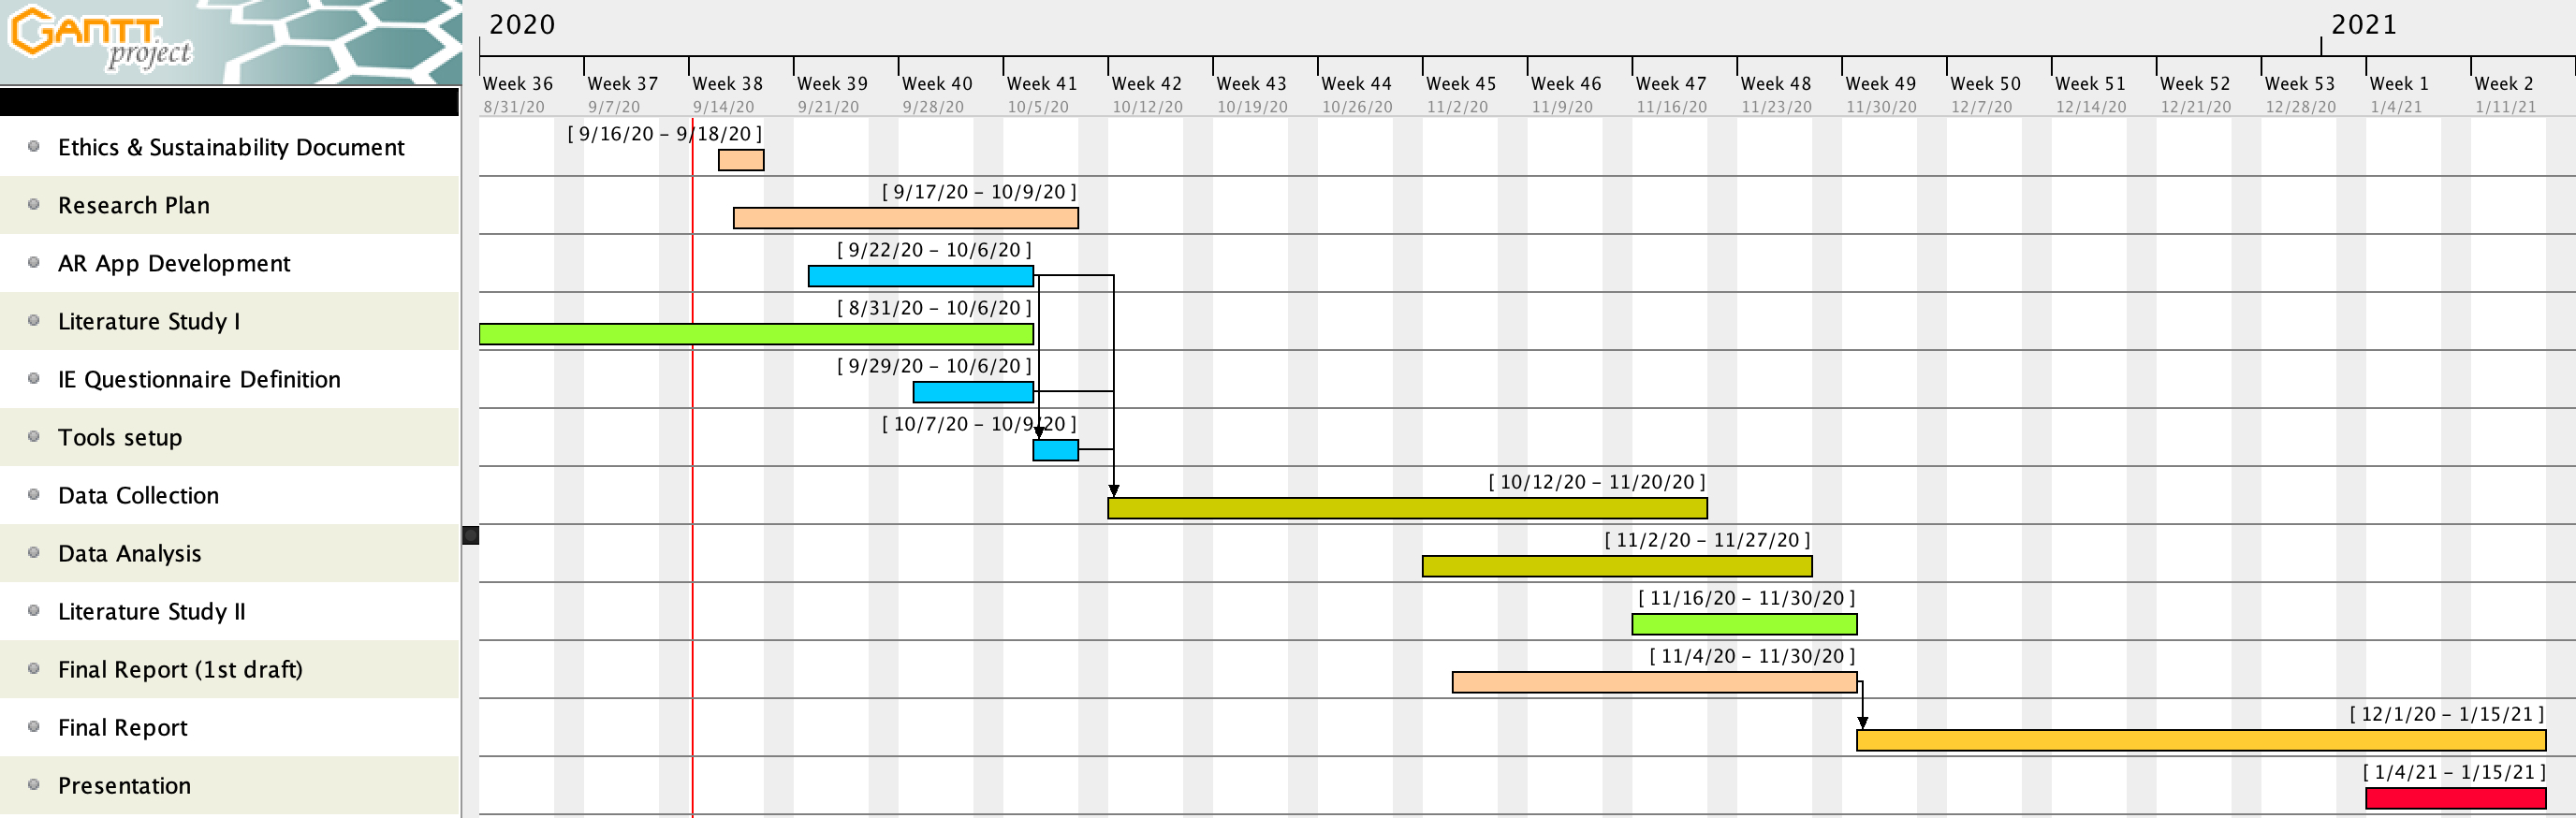
\includegraphics[width=\textwidth]{imgs/project_milestones}

\printglossary[type=\acronymtype, nonumberlist]
\clearpage
\end{document}
